% 2010 年北京卷文科第 7 题：八边形班徽（四个腰长为 1、顶角为 α 的等腰三角形 + 正方形）。
% 来源 PDF：普通高考/2010/2010北京文.pdf，SHA-256 8def639c25748266a140a99f6111811c7037bced389a451089eff7b1a0b0ba52。
% 原页：第 1 页（A3 三栏）第 1 栏下部，书页码 575。
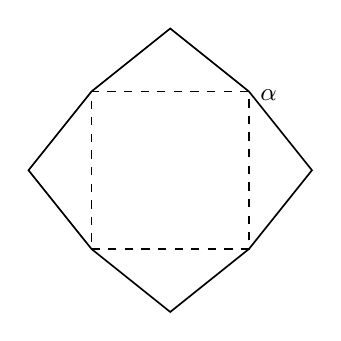
\begin{tikzpicture}[semithick, every node/.style={inner sep=1.2pt, font=\small}]
  % 正方形
  \coordinate (A) at (-1,-1);
  \coordinate (B) at (1,-1);
  \coordinate (C) at (1,1);
  \coordinate (D) at (-1,1);
  \draw[dashed] (A) -- (B) -- (C) -- (D) -- cycle;
  % 四个等腰三角形的外顶点
  \coordinate (P1) at (0,1.8);
  \coordinate (P2) at (1.8,0);
  \coordinate (P3) at (0,-1.8);
  \coordinate (P4) at (-1.8,0);
  \draw (D) -- (P1) -- (C);
  \draw (C) -- (P2) -- (B);
  \draw (B) -- (P3) -- (A);
  \draw (A) -- (P4) -- (D);
  \node at (1.25,0.95) {$\alpha$};
\end{tikzpicture}
